\clearpage
\setcounter{page}{1}
\maketitlesupplementary
\section{Per-scene results}
\TODO{per-scene tables: compression (13 scenes $\times$ 5 targets, from budgetmesh-rd-table-2026-11-10.md), vertex-cap pairs (batch24-analysis), ablation rows (batch24-analysis), capacity-limited NeRF-Synthetic rows}
\section{Size controller}
\begin{figure}[h]\centering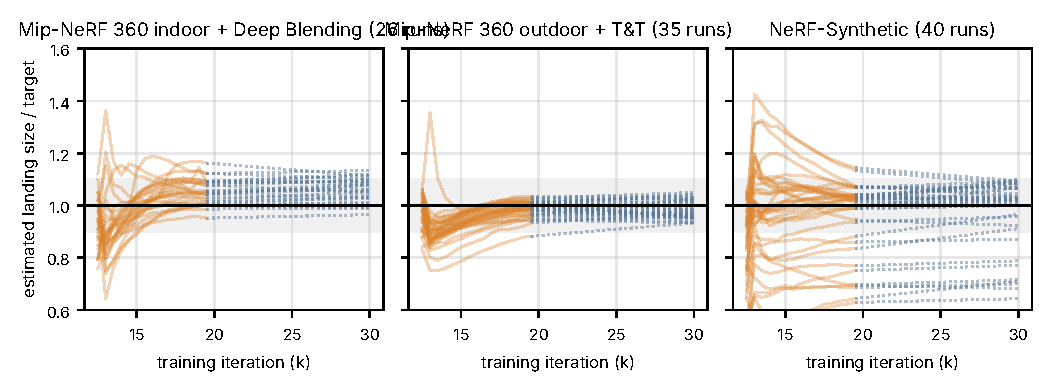
\includegraphics[width=\linewidth]{figures/fig_controller_traces.pdf}
\caption{Size controller traces for all 101 runs (89 below the capacity limit and 12 at it): the estimated landing size divided by the target at each collapse round, continued to the delivered file. Grey band: $\pm10\%$. Indoor scenes start above the target (the growth aim) and are trimmed down; outdoor scenes start below and drift up as the visible set grows; the NeRF-Synthetic runs below 0.8 are objects at the capacity limit.}\end{figure}
\begin{figure}[h]\centering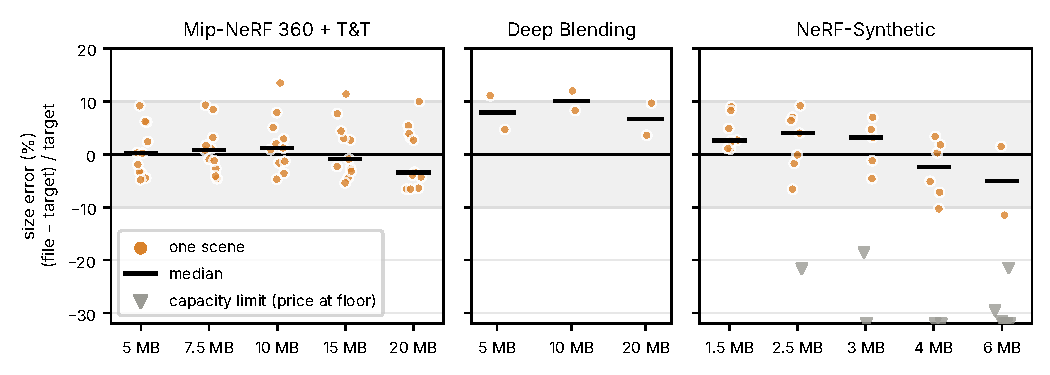
\includegraphics[width=\linewidth]{figures/fig_size_error_strip.pdf}
\caption{Size error of every run, one dot per scene, by dataset and target; black bar: median; grey band: $\pm10\%$; grey triangles: capacity-limited objects.}\end{figure}
\TODO{byte-probe accuracy (probe / delivered 0.999--1.001 on 49 runs), per-run overhead (+8--15 min), the price per growth step for one scene, growth aim 1.0 vs 1.25 on the same 33 pairs}
\section{Where the bytes go}
\begin{figure}[h]\centering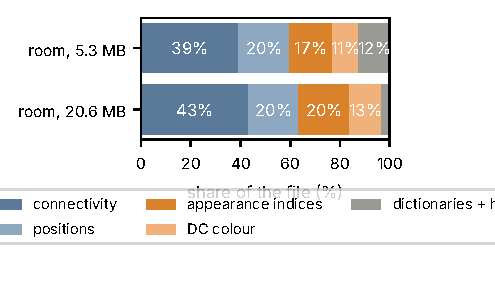
\includegraphics[width=0.9\linewidth]{figures/fig_bytes_per_stream.pdf}
\caption{Bytes per stream of a 20~MB and a 5~MB file. Connectivity and the dictionaries are lossless; the loss sits in the appearance indices and the DC color.}\label{fig:bytes}\end{figure}
\section{Size error at the remaining targets}
Mip-NeRF~360 + T\&T, 15~MB: 15.1~MB, $+0.9\%$ ($-5.4$..$+11.4$), 10/11, 23.62 ($-0.43$), 0.701 / 0.415. 7.5~MB: 7.6~MB, $+1.0\%$ ($-4.6$..$+9.3$), 11/11, 23.12 ($-0.92$), 0.669 / 0.462. NeRF-Synthetic, 3~MB: 3.1~MB, $+1.8\%$ ($-4.6$..$+7.0$), 5/5 (+2 capacity-limited), 31.10 ($-0.13$), 0.945 / 0.078; 6~MB: six of eight objects capacity-limited.
\section{Appearance dictionary sweep and DC precision}
\TODO{21 scenes $\times$ 4 prices $\times$ 6 dictionary variants; DC 8-bit rows; the $K$-should-follow-$V$ observation with the mic / ficus numbers}
\section{Generic codecs, full table}
\TODO{13 scenes, all routes, MB and PSNR, from generic-codecs-all-scenes-2026-11-10.md; Draco + our indices rows}
\section{Cross-representation figure}
\begin{figure}[h]\centering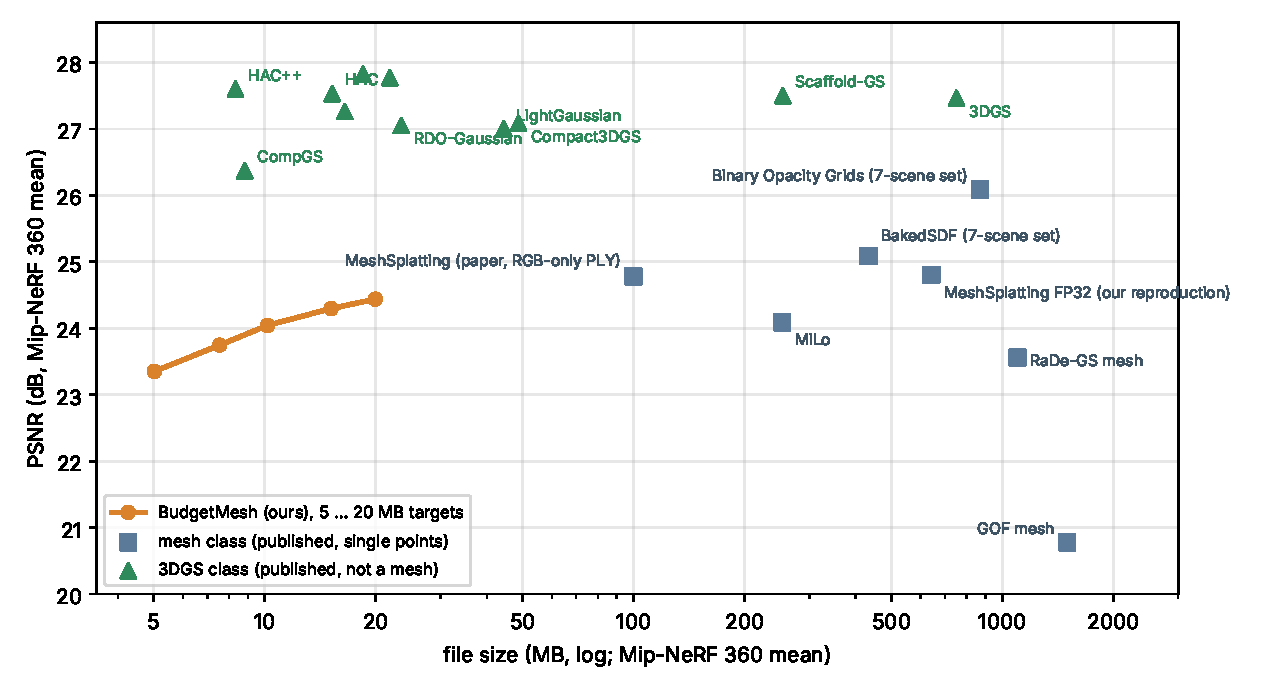
\includegraphics[width=0.9\linewidth]{figures/fig_cross_methods_mip360.pdf}
\caption{Mip-NeRF~360 means: \BM (curve) against published single points of mesh-output methods (squares) and 3DGS-class codecs (triangles).}\end{figure}
\section{Decoder and mesh statistics}
\TODO{decoder isolation test, stream list and file format; manifoldness and sliver statistics of the delivered meshes; the un-stacking measurement behind the growth aim}
